\chapter{Experiments}\label{chap:experiments}
A series of experiments were carried out to determine the performance of the network in its stated goal of classifying traversability. To this end, the network was tested on the Mapillary Vistas dataset \cite{mapillary} and its hyperparameters optimized using the Bayesian optimization with hyperband (BOHB) procedure\cite{bohb}

\section{Evaluation Metrics} \label{section:experiments-evaluationmetrics}
The mean Intersection over Union (mIoU) is the main evaluation metric chosen.
IoU measures the intersection of the prediction and the ground truth data, divided by the union of the prediction and the ground truth data.
This is formally defined as
\begin{align}
	J(A_m,B_m) &= \frac{|A_m \cap B_m|}{|A_m \cup B_m|}
\end{align}
where $A$ is the prediction, $B$ the ground truth, and $m$ the class.
The mIoU is thus defined as
\begin{align}
	J(A,B) &= \frac{1}{|m|} \sum_{m}\frac{|A_m \cap B_m|}{|A_m \cup B_m|}
\end{align}
and can be intuitively understood as the average of the class-wise IoU accuracy values.

\section{Dataset} \label{section:experiments-dataset}
We evaluate our approach on the Mapillary Vistas dataset as it was, to our knowledge, the only street-level dataset that included ground truth segmentations of both curbs and curb cuts at the time of writing.
This dataset contains images from all around the world and includes images captured from different imaging devices including mobile phones, action cameras, and professional imaging solutions.
These images are captured during various weather, seasonal, and daylight conditions.
As such, the dataset provides a challenging level of diversity.

Some image samples from the dataset can be seen in \figref{fig:experiments-datasetsamples}.
These images show some examples of how diverse the images in the dataset can be.
The dataset also contains images taken from sidewalks, such as in the case of Figure \ref{fig:dataset-3}.
This is especially useful for our end goal of training a segmentation network for an autonomous pedestrian robot.
The diversity of the dataset improves the generalizability of our model.

\begin{figure}[]
	\centering
	\begin{subfigure}{.45\textwidth}
		\centering
		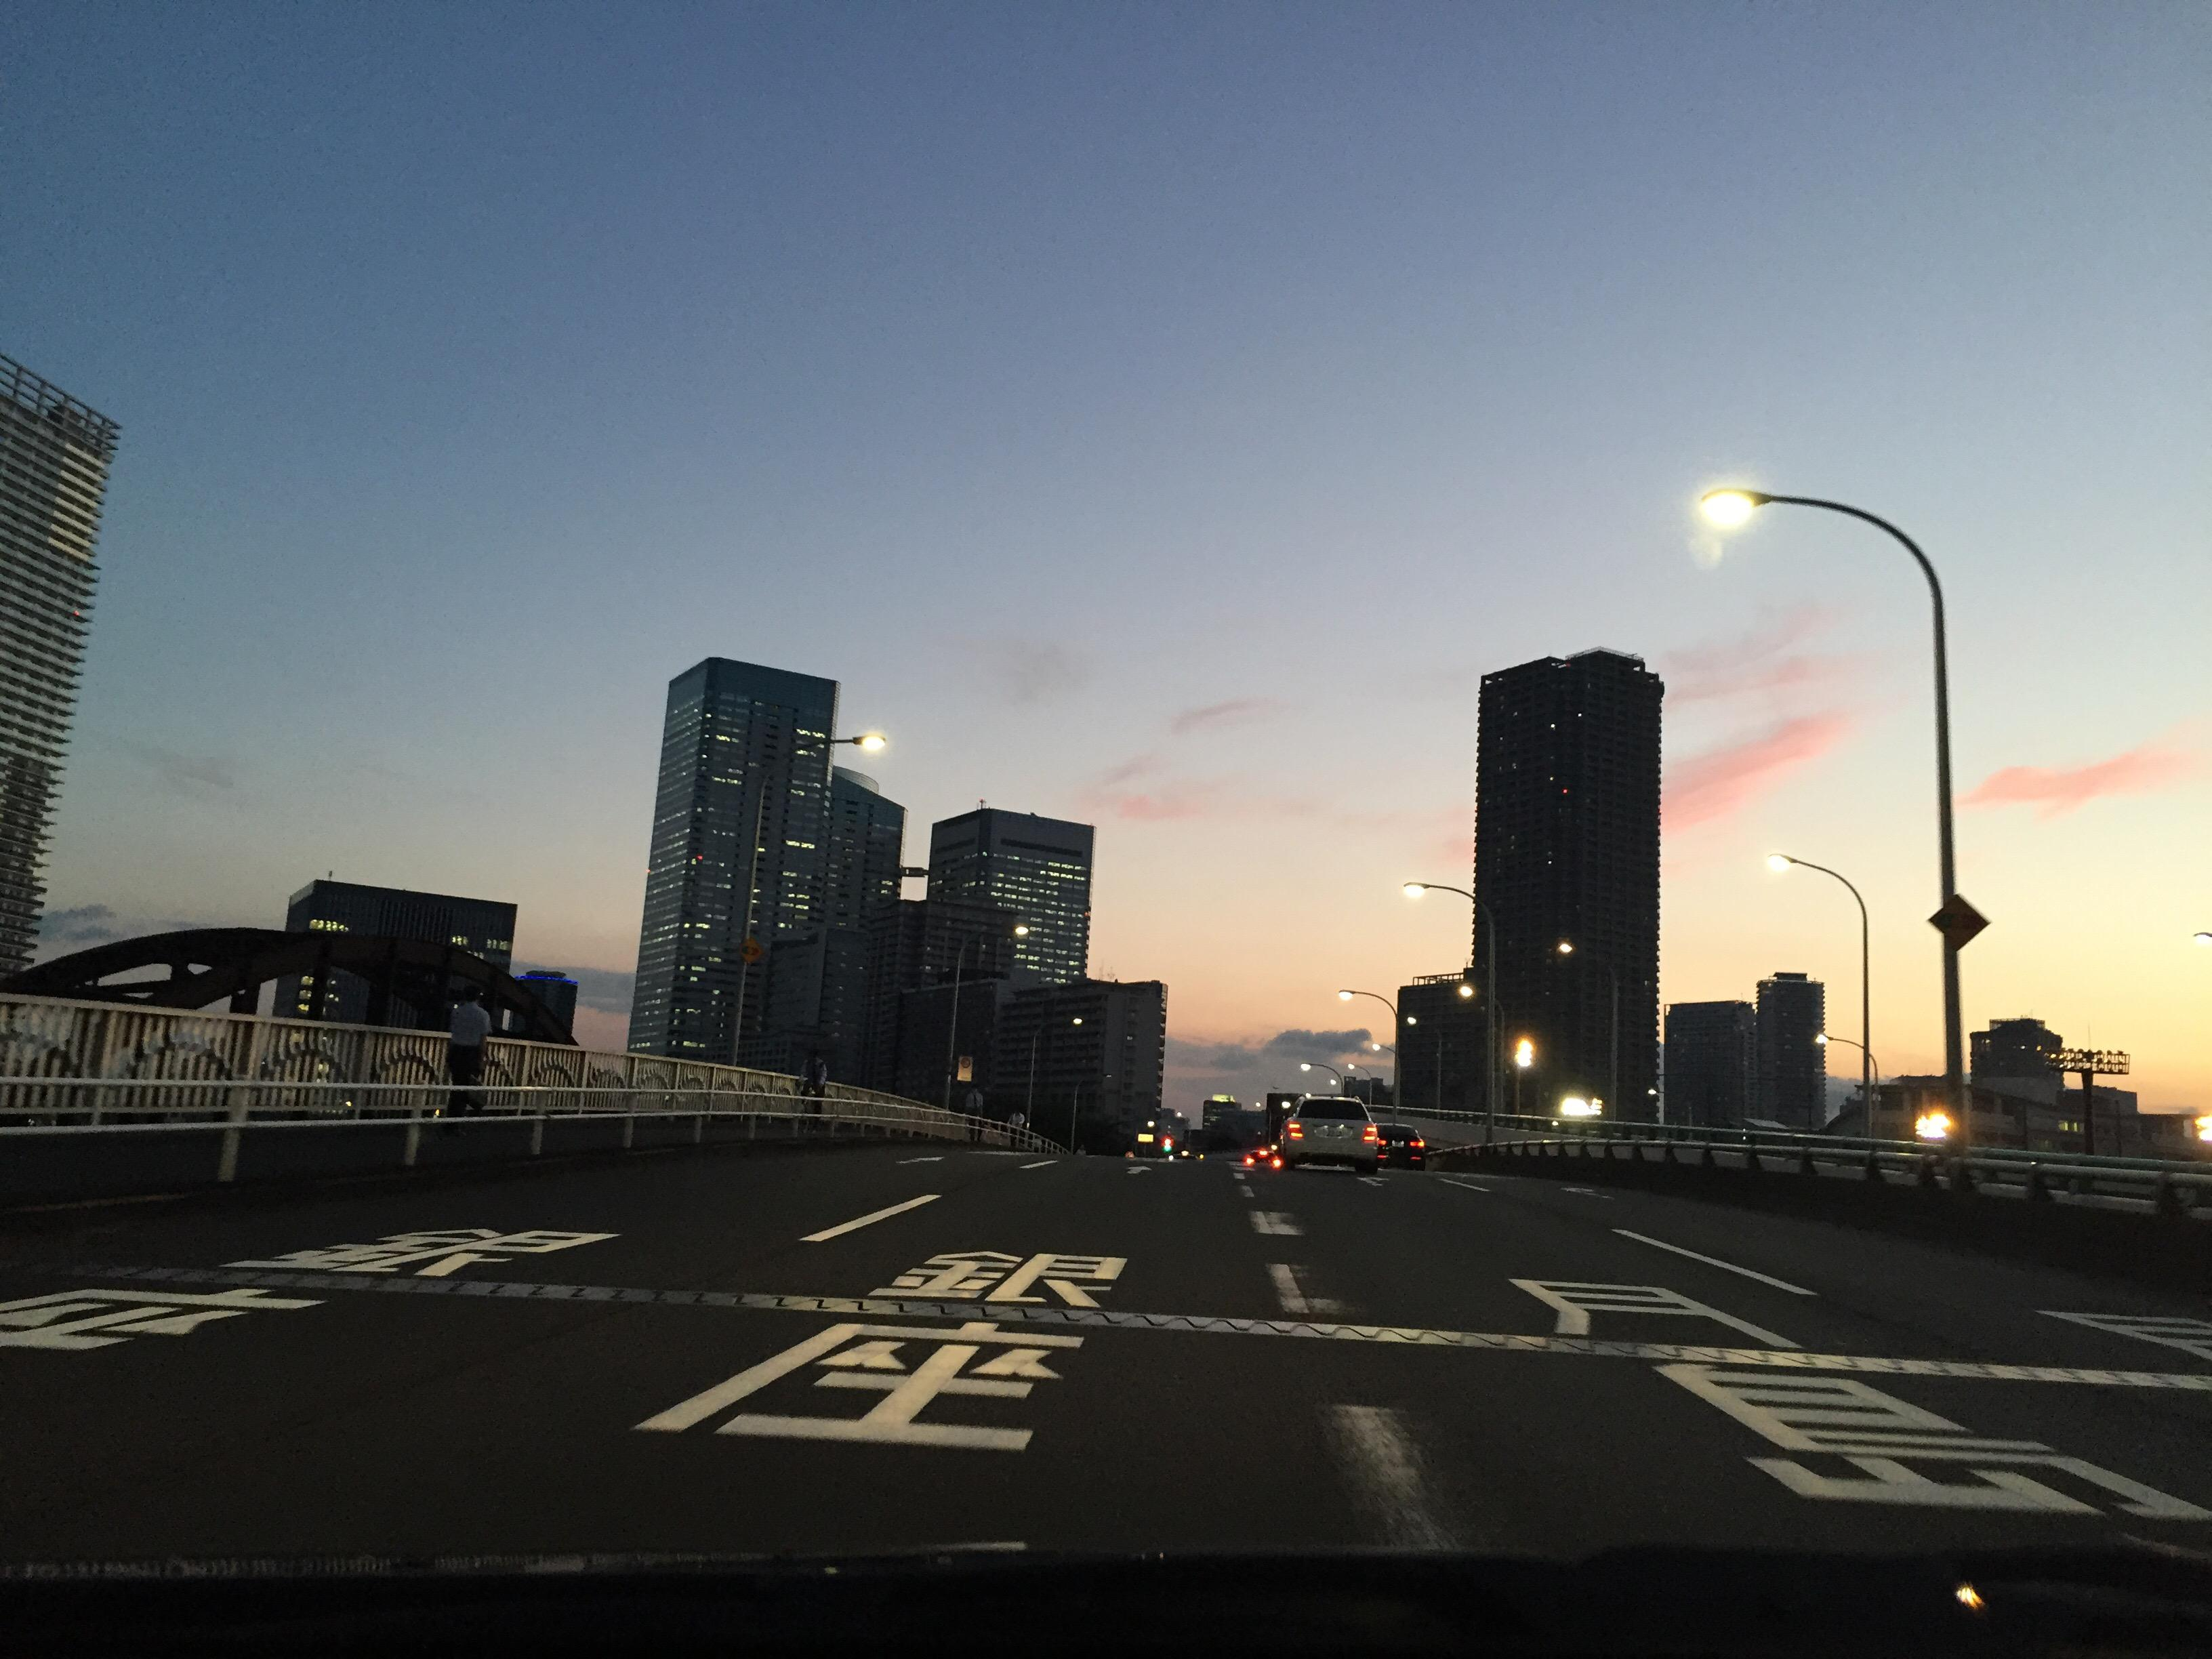
\includegraphics[width=\linewidth]{figures/experiments/dataset/1.jpg}
		\caption[Dataset Sample 1]{This image shows an axample of an evening scene.}
		\label{fig:dataset-1}
	\end{subfigure}
	\hfill
	\begin{subfigure}{.45\textwidth}
		\centering
		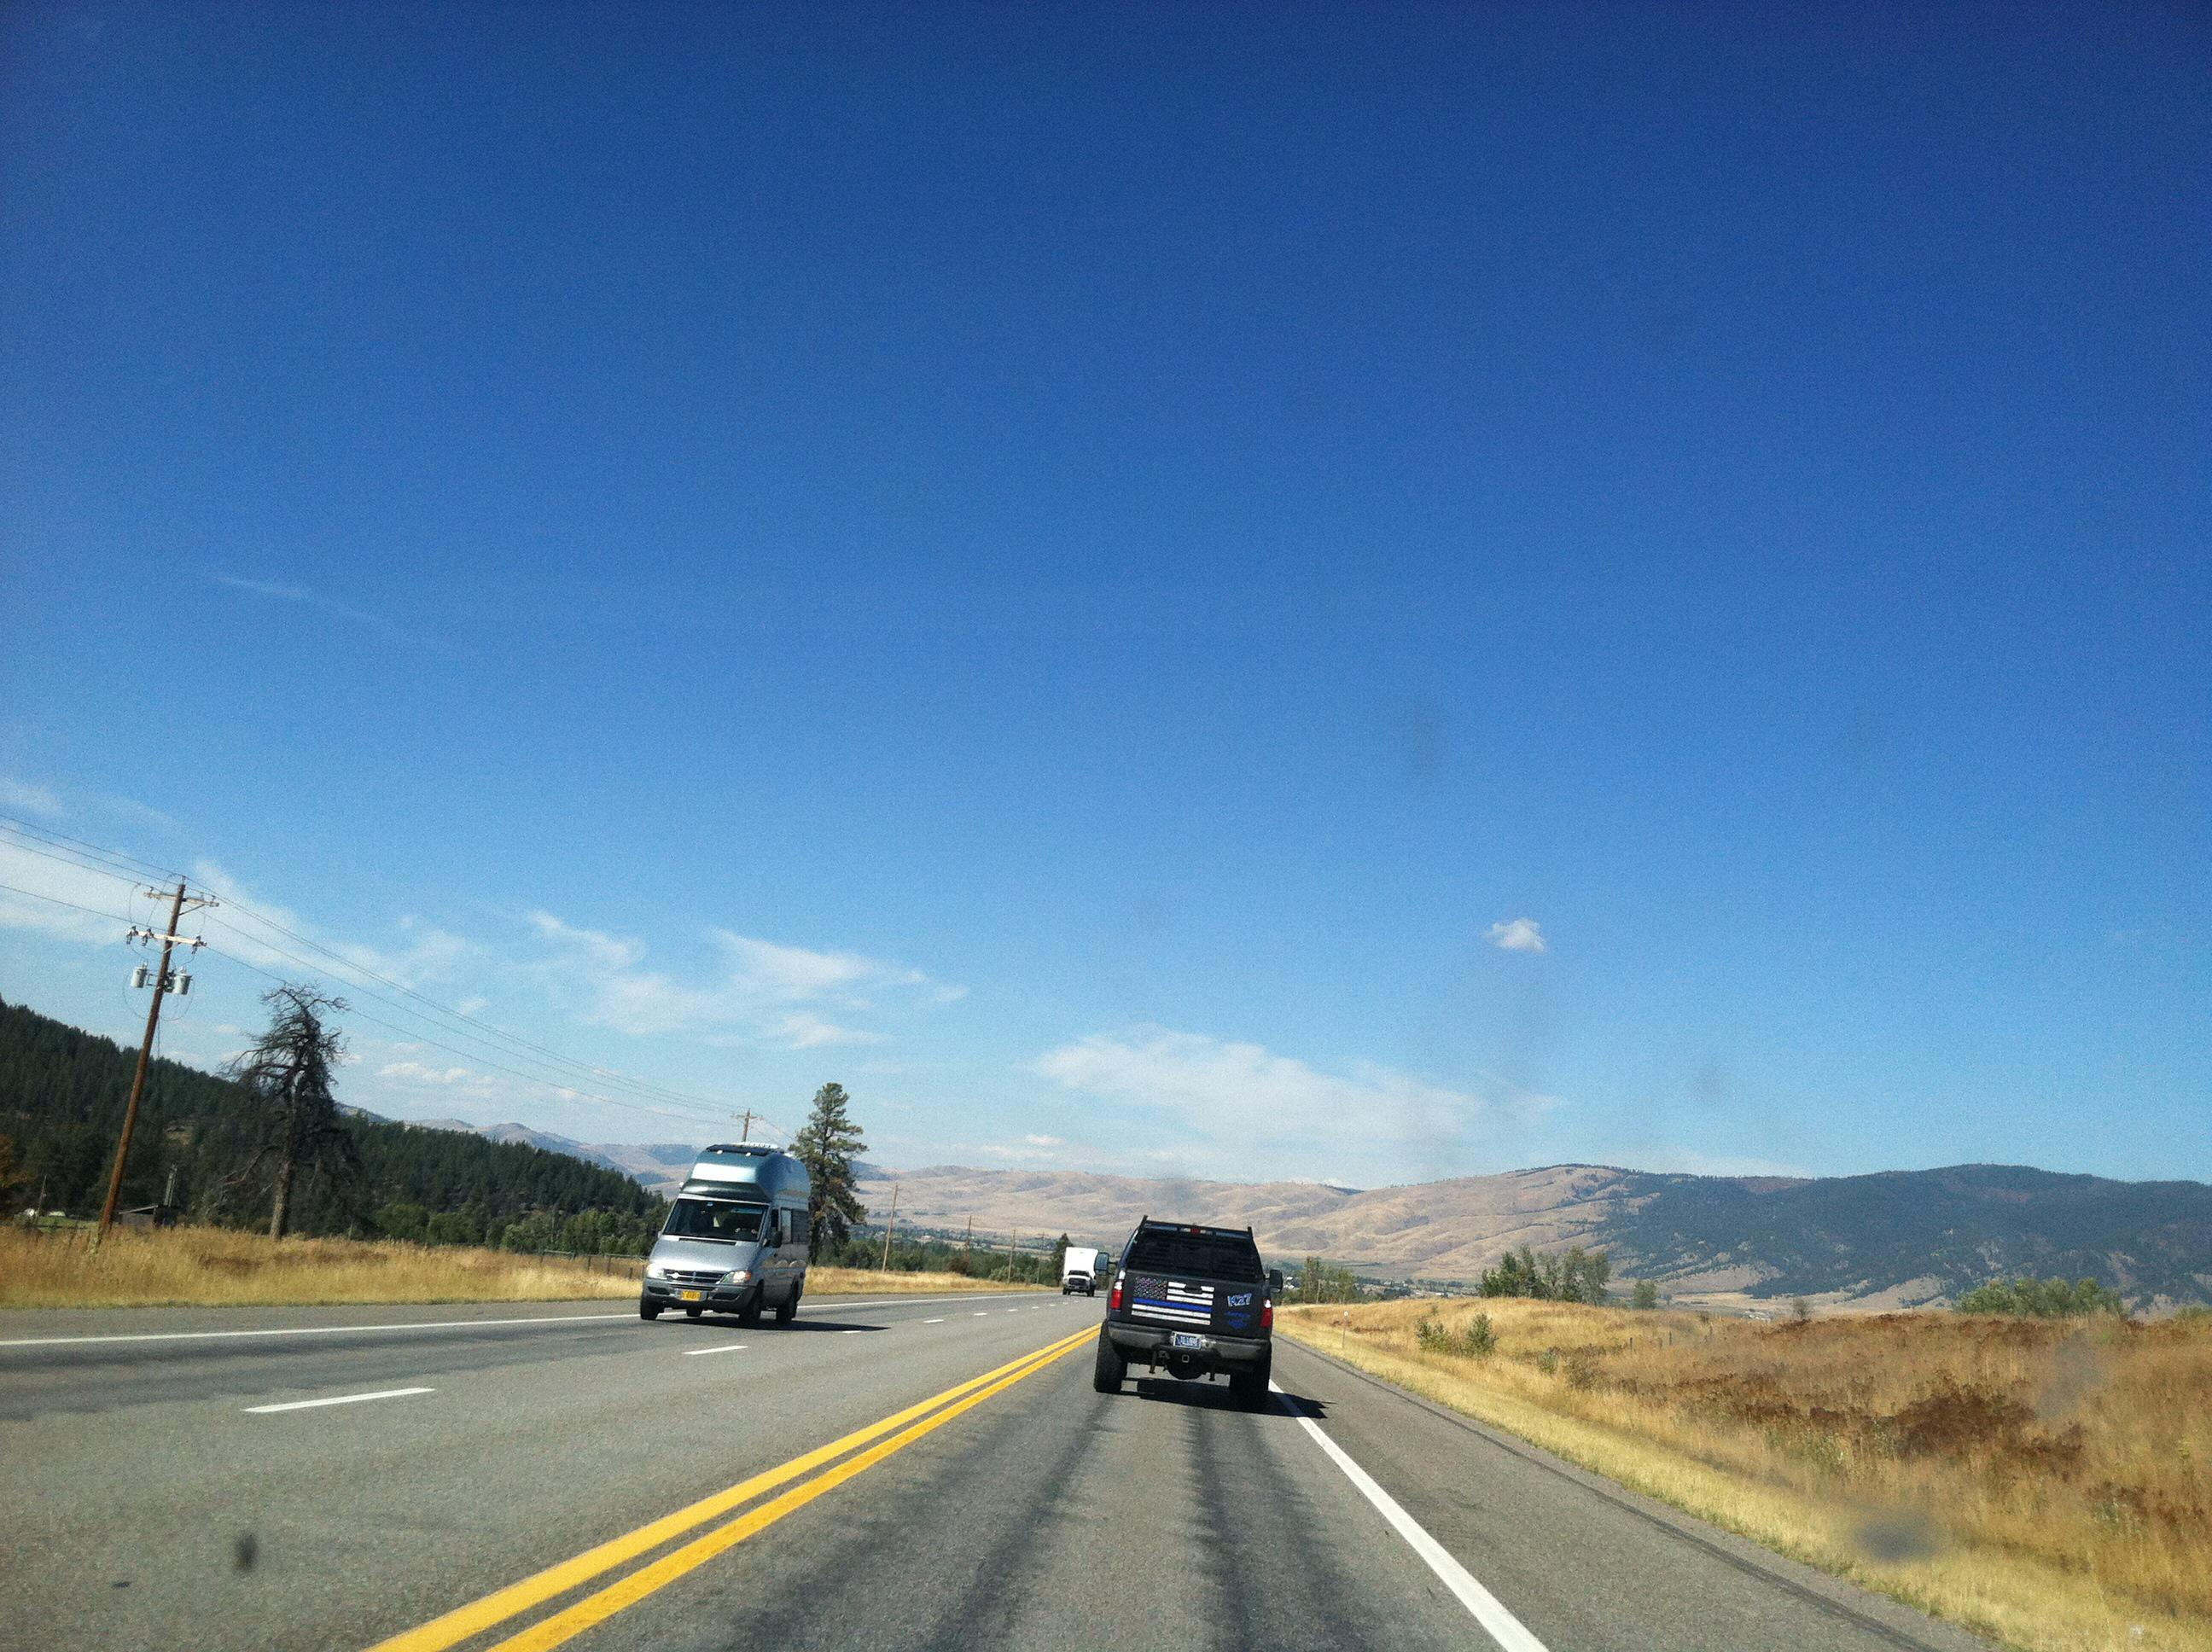
\includegraphics[width=\linewidth]{figures/experiments/dataset/2.jpg}
		\caption[Dataset Sample 2]{This image shows an example of a very bright scene in a rural area.}
		\label{fig:dataset-2}
	\end{subfigure}
	
	\vspace{12pt}%------------ 
	
	\begin{subfigure}{.45\textwidth}
		\centering
		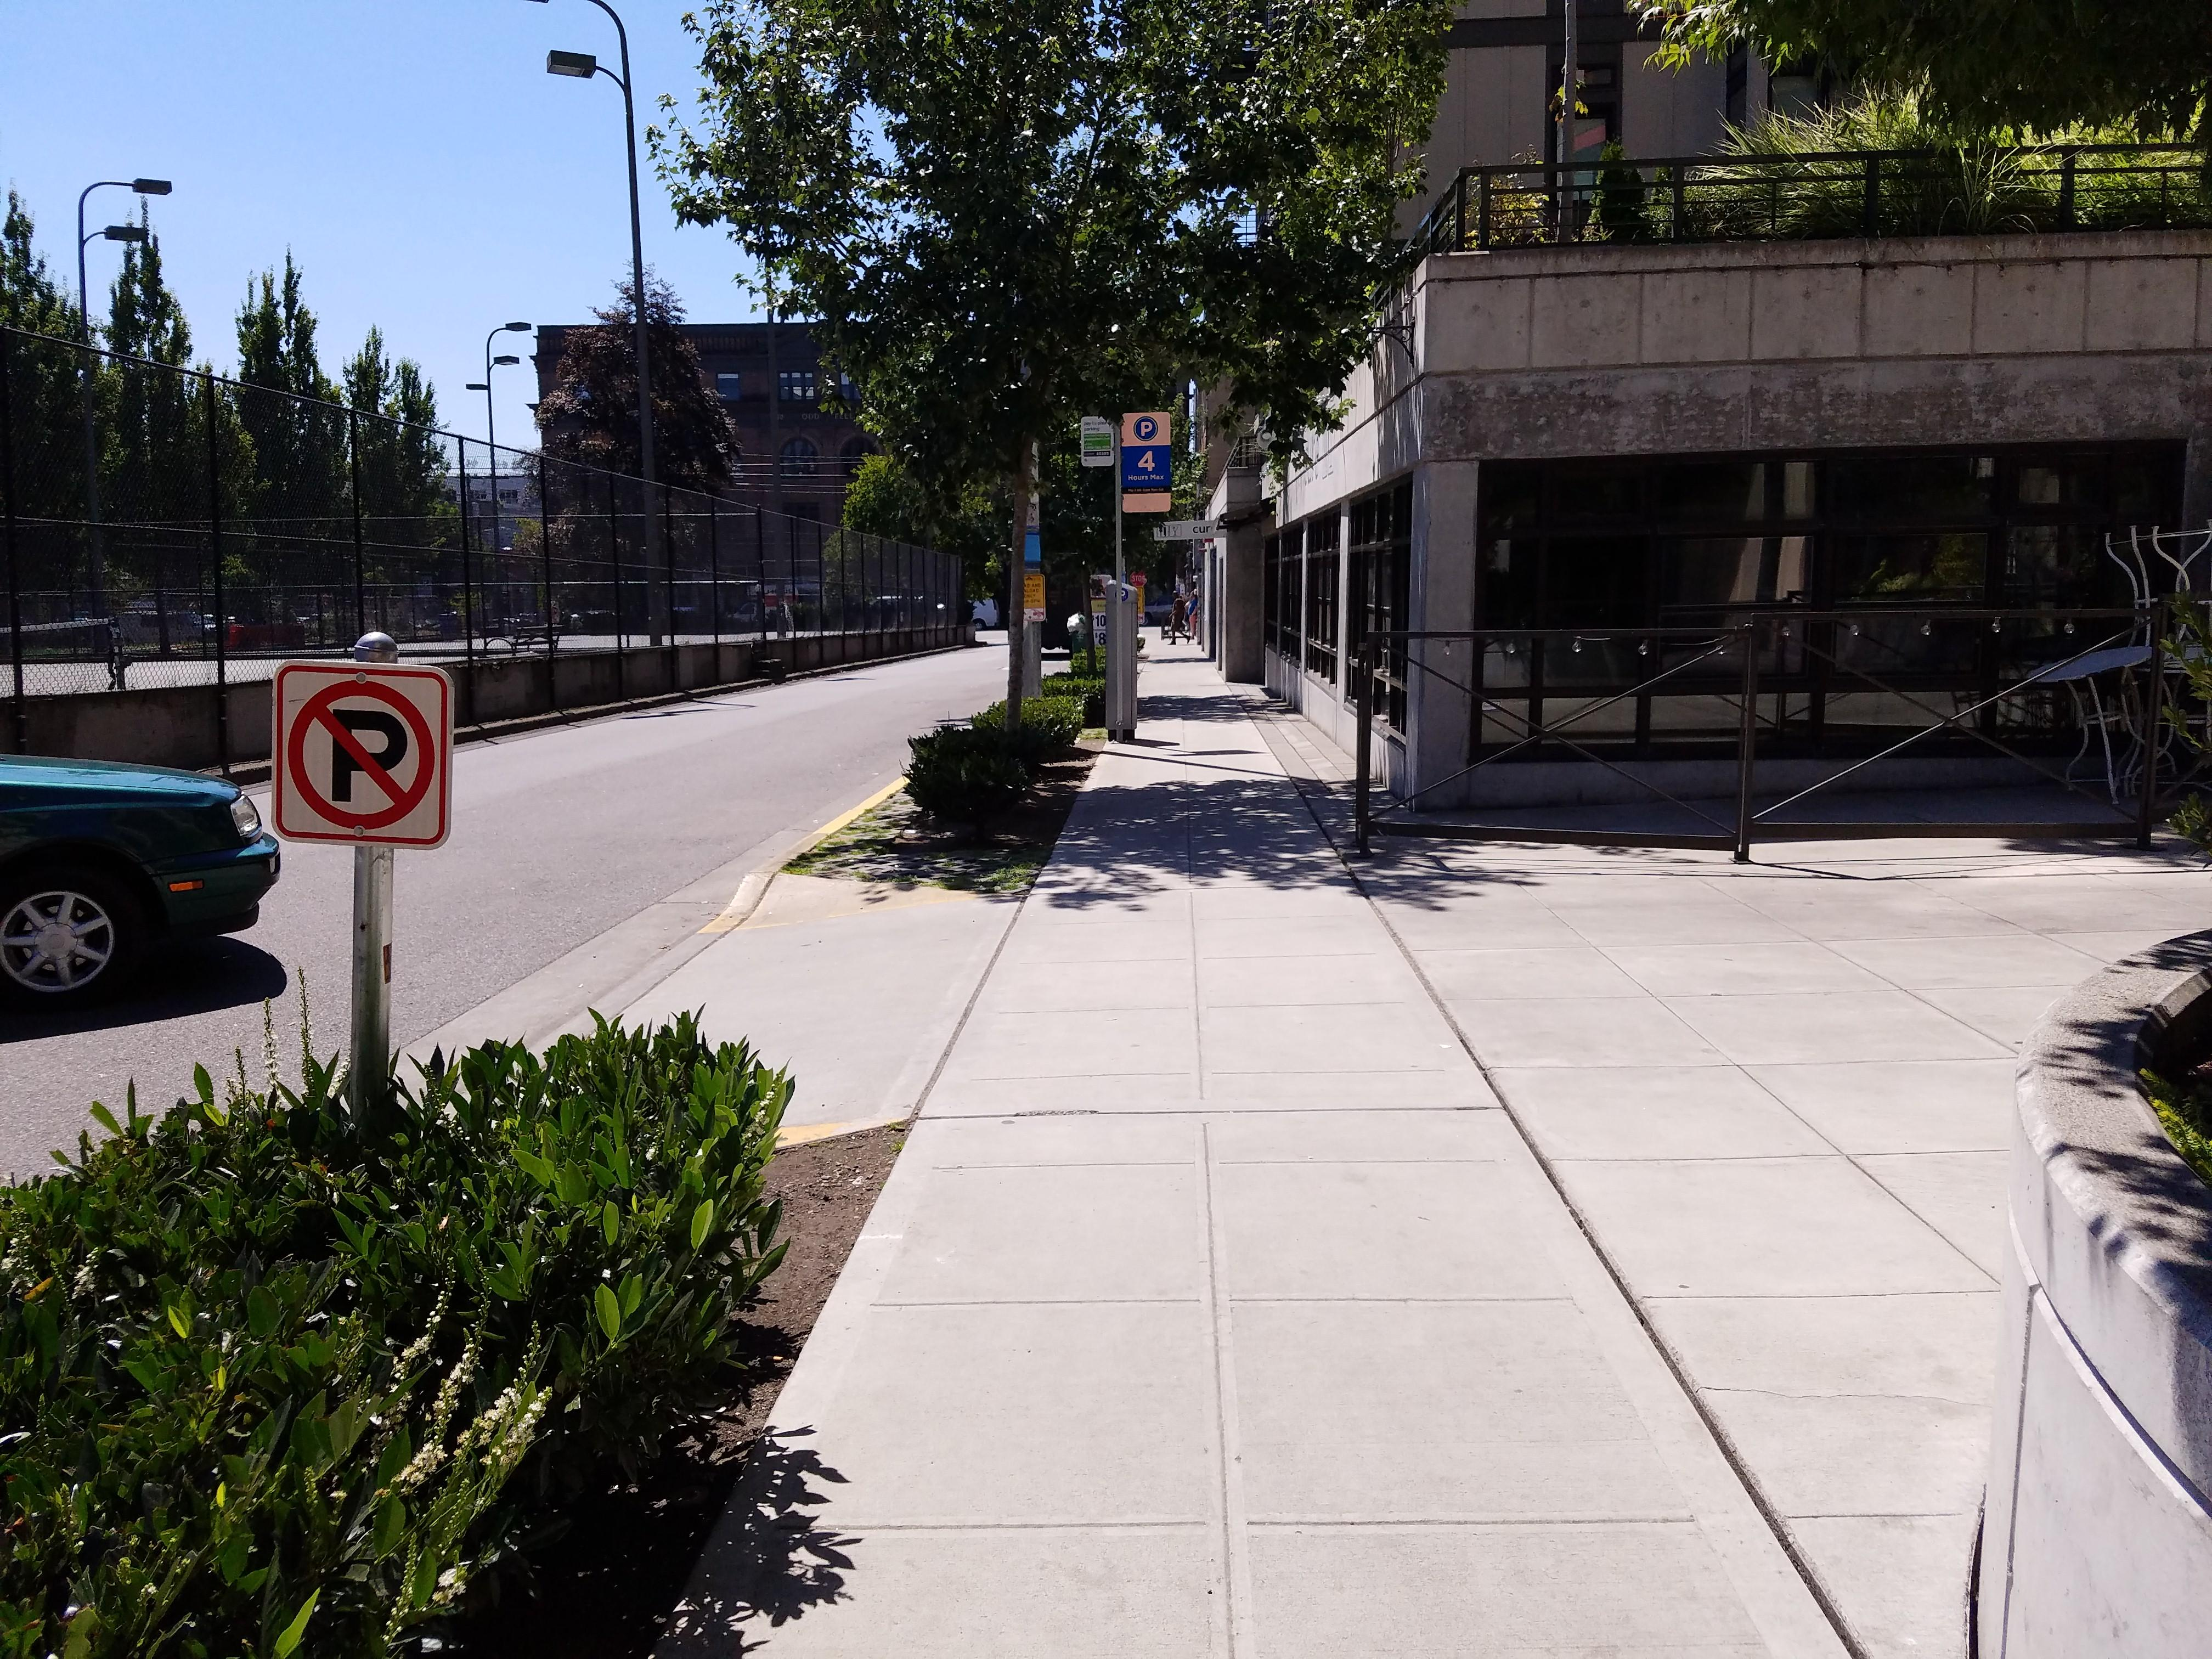
\includegraphics[width=\linewidth]{figures/experiments/dataset/3.jpg}
		\caption[Dataset Sample 3]{This image shows an example of an image from a sidewalk.}
		\label{fig:dataset-3}
	\end{subfigure}
	\hfill
	\begin{subfigure}{.45\textwidth}
		\centering
		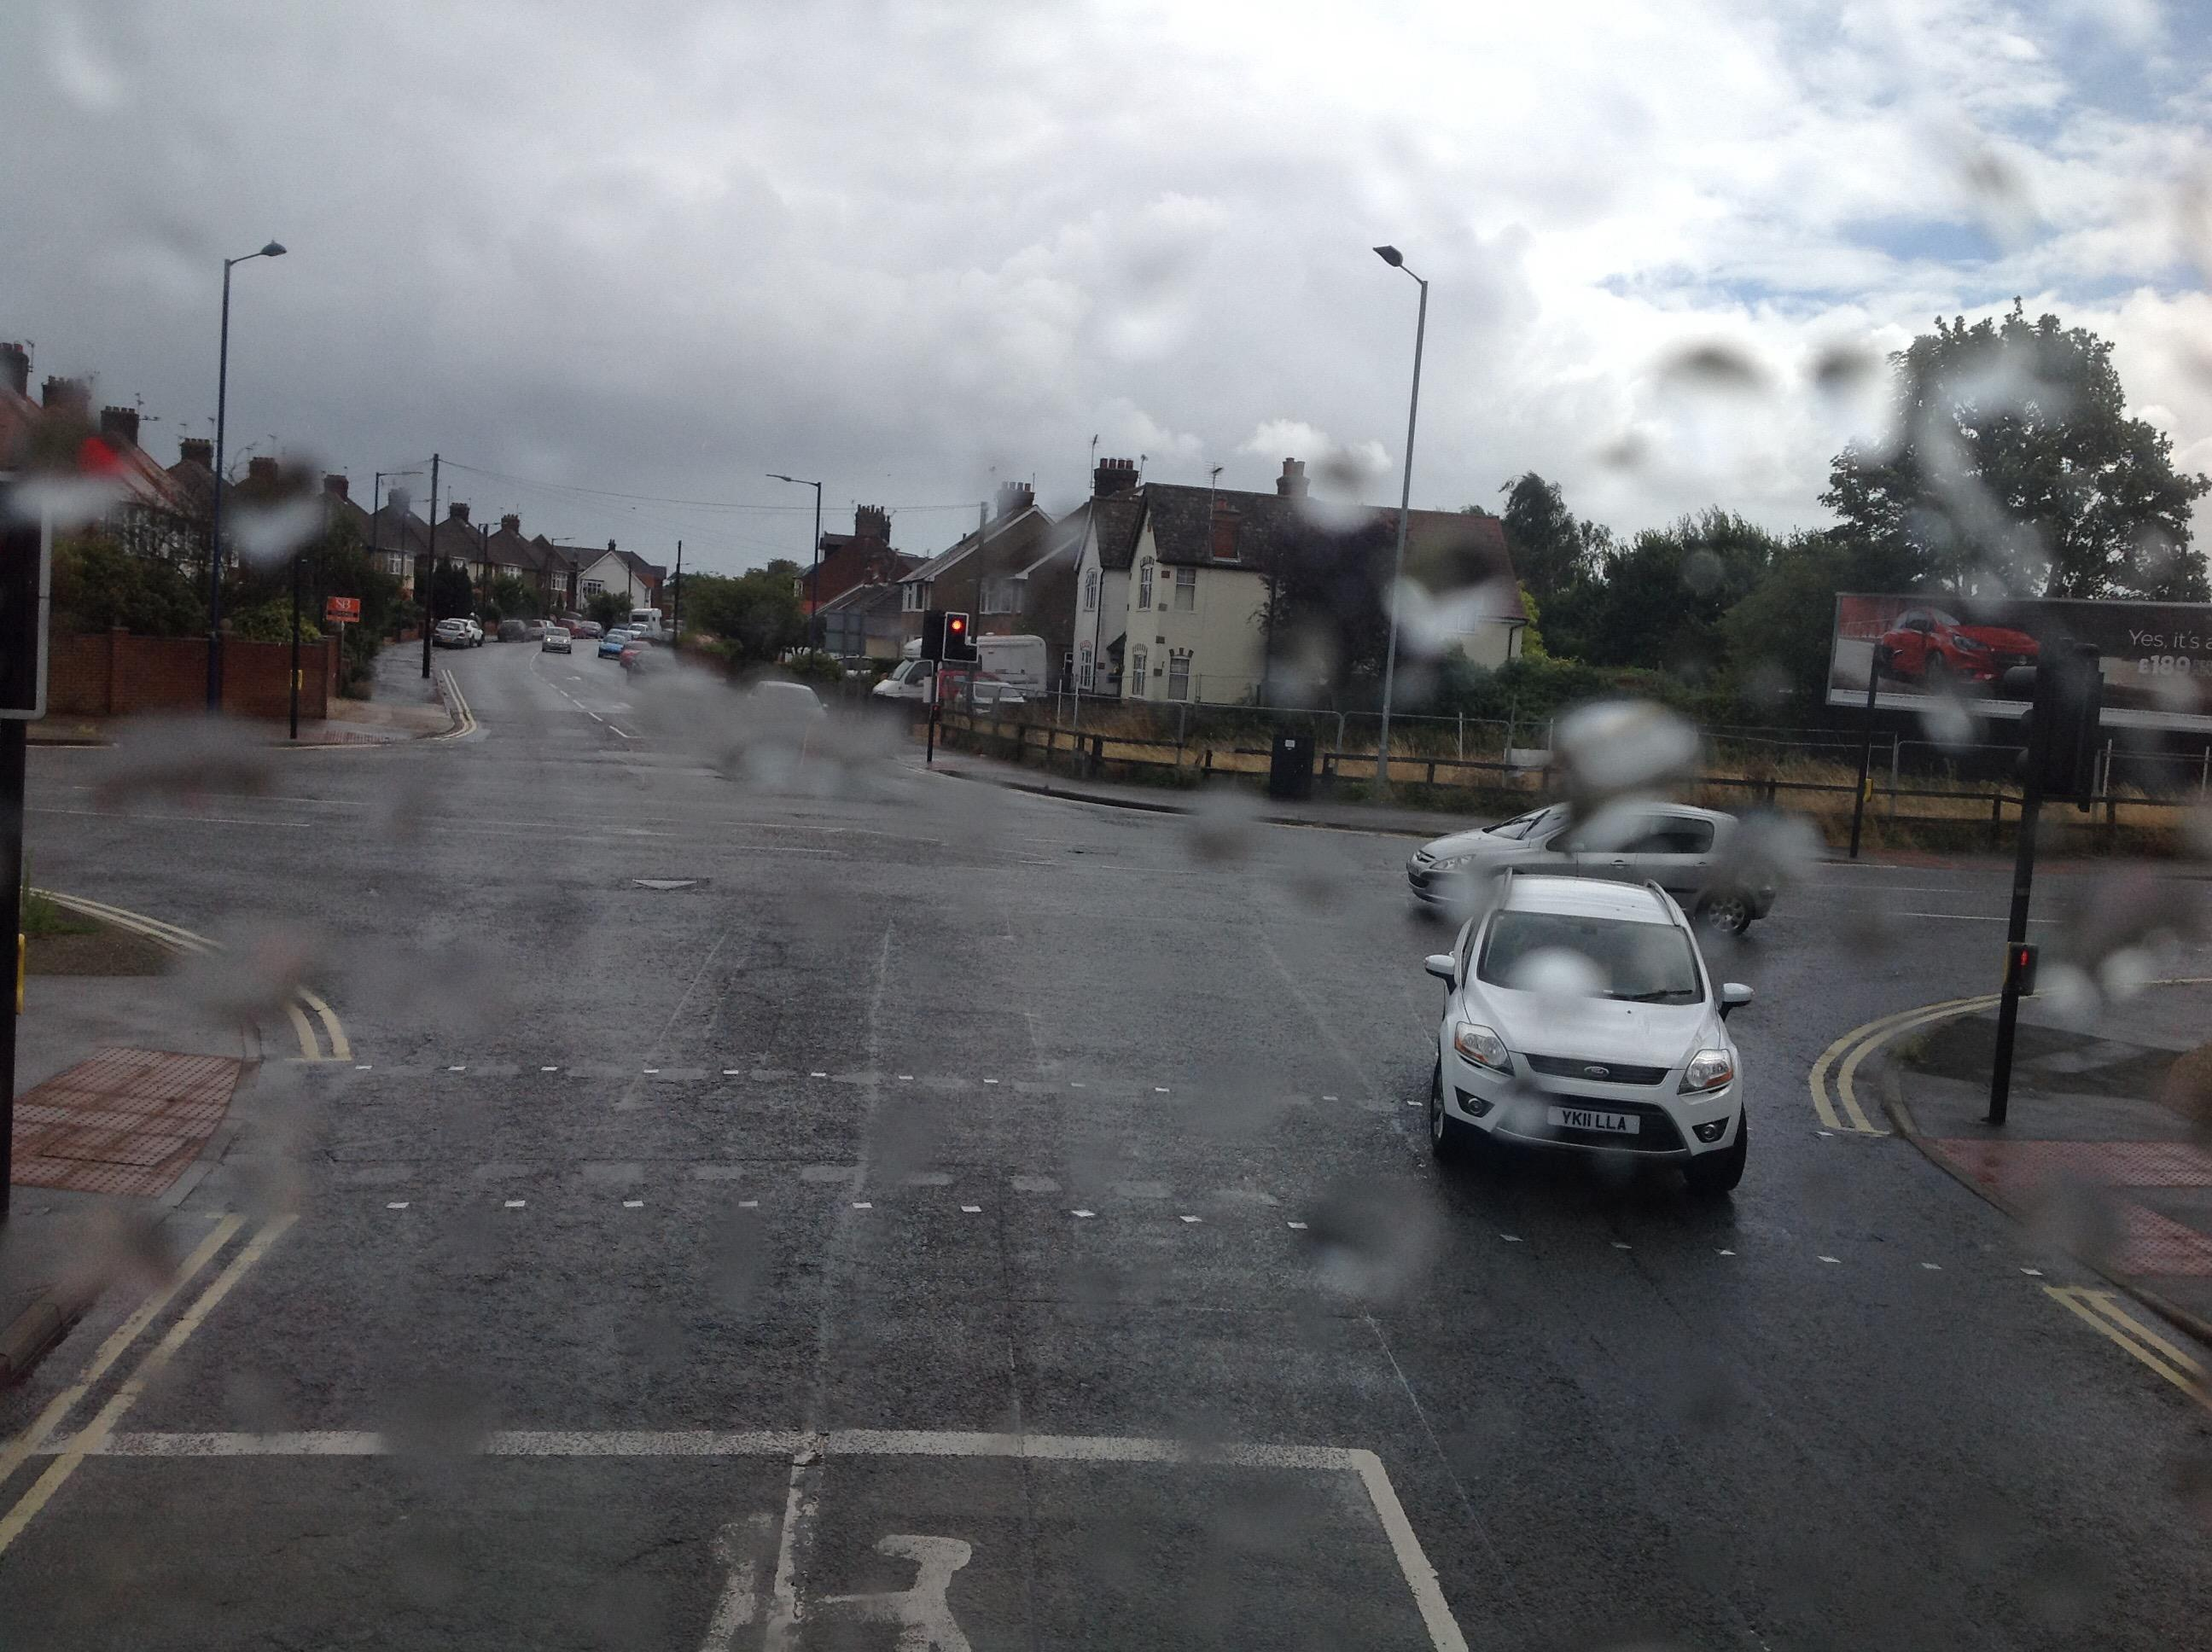
\includegraphics[width=\linewidth]{figures/experiments/dataset/4.jpg}
		\caption[Dataset Sample 4]{This image shows an example of an image taken during rainy conditions.}
		\label{fig:dataset-4}
	\end{subfigure}

	\caption[Mapillary Vistas Dataset Sample Images]{These sample images from the Mapillary dataset shows how varied and diverse the dataset is. This diversity makes the dataset an excellent choice in training a network that can generalize to unseen conditions.}
	\label{fig:experiments-datasetsamples}
\end{figure}

The image dimensions in the dataset are also not standardized, with 156 different image dimensions ranging from $(640 \times 480)$ to $(6528 \times 5248)$. 
With such a diverse range of dimensions, the images must first be preprocessed.
We process all the images to conform to a 4:3 size ratio, eliminate images without images of curbs or curb cuts, and extract only road, curb, and curb cut classes.

To optimize training speed with respect to wall clock time, and given the computational constraints, images were resized for training.
The chosen image resolution was $360 \times 320$ pixels. 
We use an NVIDIA Titan X GPU with 12 GB of VRAM.
This allows a batch size of 16 per GPU.
To further optimize training, the images are resized prior to training and the resized images stored.
This allows all training and validation images to be loaded into memory once at the beginning of training, reducing the number of file accesses required and reducing training wall clock time by a factor of two.

After running an analysis of the dataset with respect to their curb and curb cut content and image dimensions, we found that there were 15,160 usable images in the training set and 1610 usable images in the validation set.
Usable images in this case refers to images that at least contain both curbs and curb cuts.
A detailed results of the analysis of the dataset can be found in Appendix section \ref{appendix:dataset}.

We also applied image augmentation to our dataset.
The augmentations we have applied are Gaussian blur, dropout, brightness adjustment, and contrast adjustment.

\section{Network Evaluation}\label{section:experiments-networkevaluation}
Experiments were done to evaluate the performance of different networks on our dataset.
Specifically, we identified the small size of curbs relative to the rest of the image causes a severe class imbalance and increases the difficulty in recognizing the smaller features.

Relative to the entire image, curb and curb cut classes make up a relatively small proportion of the image, making up an average of 0.986\% and 0.196\% of images respectively.
As such, three networks with good known performance for urban scene segmentation were chosen and evaluated for their performance classifying traversability classes.
We experimented with GoogLeNet, described in the paper "Going Deeper with Convolutions"~\cite{googlenet}; FCN16s, described in "Fully Convolutional Networks for Semantic Segmentation"~\cite{fcn}; and DeepLab v3+, described in the paper "Encoder-Decoder with Atrous Separable Convolution for Semantic Image Segmentation"~\cite{deeplab}.

To evaluate which network would have the most potential, we trained each network on a small subset of the whole dataset to find which networks would yield the highest overall accuracy given a certain budget.
We use a subset of 64 images, sampled randomly from the Mapillary Vistas training subset, for training and a subset of 64 images, also sampled randomly from the Mapillary Vistas validation subset, for validation.
For each of these runs, the default recommended hyperparameters from the DeepLab v3+ paper were used.
Due to time constraints, conduct hyperparameter optimization was not done on each of the tested networks.
The results can be seen in \figref{chart:experiments-networkcomparison} and in \tabref{tab:network-comparison}.

We observe that DeepLab v3+ starts with the lowest mIoU performance but quickly achieves 28.61\% mIoU accuracy after only 80 iterations, already outperforming the final result of GoogLeNet, after which training begins to plateau.
After 1000 iterations, it was able to achieve 30.83\% mIoU accuracy.
GoogLeNet is able to also train relatively quickly, achieving 22.05\% mIoU accuracy after 80 iterations, after which performance also began to plateau achieving a final 25.08\% mIoU accuracy.
FCN16s was able to achieve 19.97\% mIoU overall after 1000 iterations.
We believe this may be due to FCN16s not being designed to identify smaller structures and features, such as in the case of curbs and curb cuts.

Given these results, we chose to use DeepLab v3+ as our network.

% Please add the following required packages to your document preamble:
% \usepackage{booktabs}
% \usepackage{graphicx}
\begin{table}[b]
	\centering
	\begin{tabular}{@{}ll@{}}
		\toprule
		Network     & mIoU \\ \midrule
		DeepLab v3+ & 30.83\%   \\
		FCN16s      & 19.97\%   \\
		GoogLeNet   & 25.08\%   \\ \bottomrule
	\end{tabular}
	\caption[Network Comparison Results]{Results of running the DeepLab v3+, FCN16s, and GoogLeNet on a subset of the main dataset after one thousand iterations. It can be seen that DeepLab v3+ was able to achieve the highest mIoU performance overall.}
	\label{tab:network-comparison}
\end{table}
\begin{figure}
	\centering
	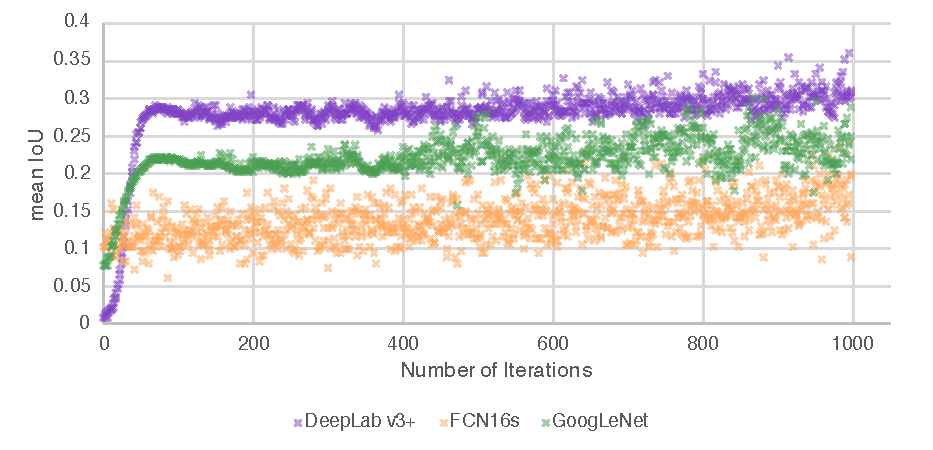
\includegraphics[width=\textwidth]{figures/experiments/network-comparison.pdf}
		\caption[Network Comparison Chart]{Training mIoU Accuracy over 1000 Iterations using DeepLab v3+, FCN16s, and GoogLeNet. It can be seen that DeepLab v3+ achieves the best mIoU performance overall.}
		\label{chart:experiments-networkcomparison}
\end{figure}

\section{Loss Function Evaluation}\label{section:experiments-loss}
Our custom loss function masked cross entropy (MCE) loss was evaluated against weighted cross entropy (WCE) loss.
We evaluated the two loss functions using the same network hyperparameters and a pretrained backbone.
The backbone is pretrained on the ImageNet database, published in 2009 by J. Deng et al~\cite{imagenet}.
Training results, shown in \figref{chart:experiments-losstraining}, show that both lost functions show similar results until the 40\textsuperscript{th} iteration, after which the network using MCE loss is able to produce better results.
Validation accuracy is plotted in \figref{chart:experiments-lossvalidation}.
We observe the validation accuracy to be similar for the first 2370 iterations.
After this point, MCE loss shows a clear advantage in validation accuracy compared to WCE loss.
After 4740 iterations, a clear performance advantage can be seen, with a difference of 5.56 mIoU percentage points.
As such, we have chosen to implement our network using MCE loss as our loss function.

\begin{figure}
	\centering
	\begin{subfigure}{\textwidth}
		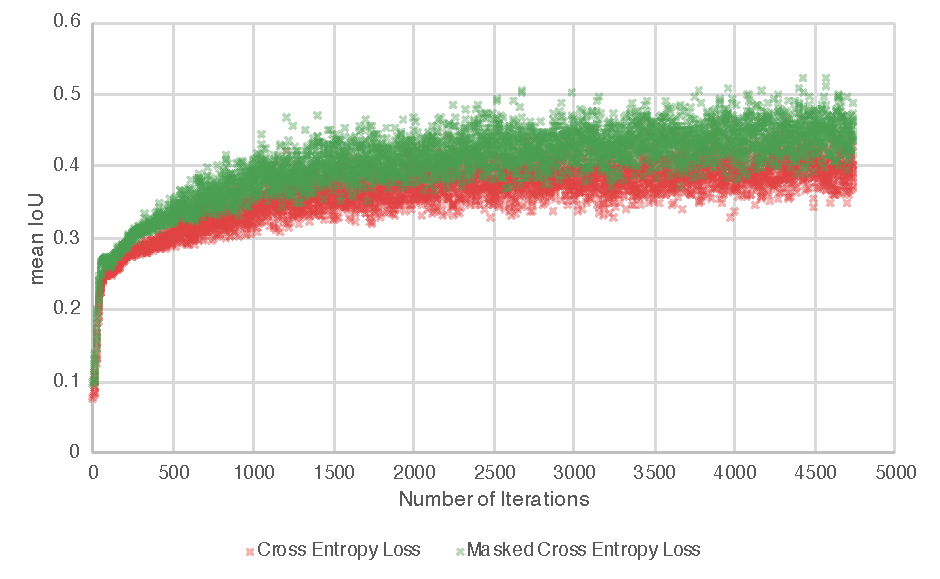
\includegraphics[width=\textwidth]{figures/experiments/loss-comparison-training.pdf}
		\caption[Loss Comparison Chart: Training]{Training mIoU Accuracy over 4740 Iterations comparing weighted cross entropy loss and masked cross entropy loss. The results show that although performing similarly to begin with, masked cross entropy loss was able to outperform weighted cross entropy loss.}
		\label{chart:experiments-losstraining}
	\end{subfigure}
	\newline
	\begin{subfigure}{\textwidth}
		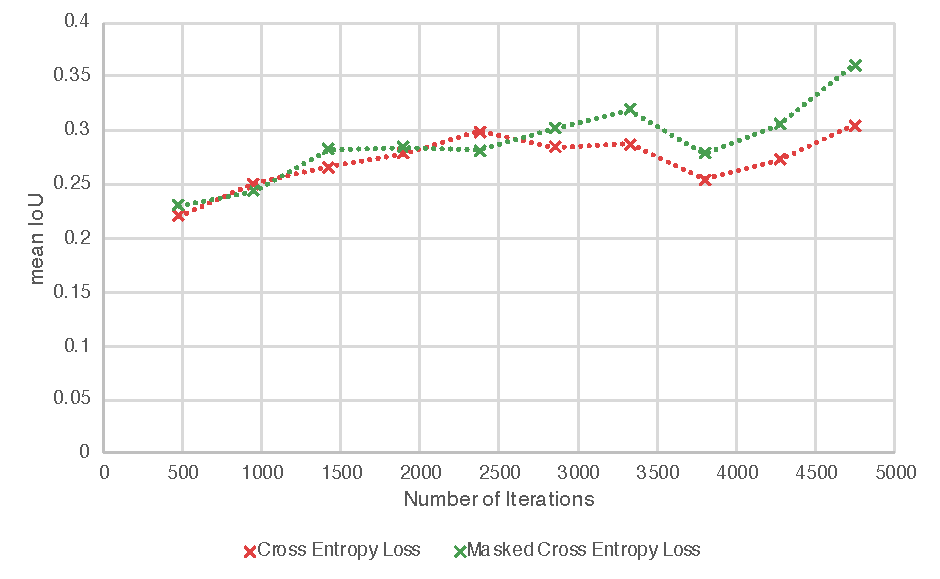
\includegraphics[width=\textwidth]{figures/experiments/loss-comparison-validation.pdf}
		\caption[Loss Comparison Chart: Validation]{Validation mean IoU Accuracy over 4740 Iterations, measured every 474 iterations, comparing cross entropy loss and masked cross entropy loss. Validation accuracy was evaluated against a validation set of 1680 images. The lines shown in the chart are to emphasize the data.}
		\label{chart:experiments-lossvalidation}
	\end{subfigure}
	\caption[Loss Comparison Chart]{Comparisons of masked cross entropy loss and weighted cross entropy loss. Both loss functions were evaluated using the same hyperparameters against a dataset consisting of 15160 training images and 1680 validation images.}
\end{figure}

\section{Hyperparameters} \label{section:experiments-hyperparameters}
Hyperparameter tuning was done by using Bayesian Optimization with HyperBand.
The hyperparameters that were tuned were the learning rate; optimizer; momentum, if the optimizer chosen was stochastic gradient descent; epsilon, if the optimizer chosen was Adam; and the loss criterion.

The learning rate is optimized between the interval $\left[1 \times 10^{-5}, 1 \times 10^{-2}\right]$, varied on a logarithmic scale.
The optimizer is a categorical choice between stochastic gradient descent or Adam.
The momentum is optimized between the interval $\left[0, 0.99\right]$.
The epsilon value is optimized between the interval $\left[1 \times 10^{-2}, 1\right]$.
The weight ratio for the loss weight determines the ratio of the weights between the curb and curb cut.
The loss criterion is a categorical choice between weighted cross entropy loss or masked cross entropy loss.
Further details of the hyperparameters optimized can be found in \tabref{tab:hyperparameters}.

% Please add the following required packages to your document preamble:
% \usepackage{booktabs}
\begin{table}[]
\begin{tabular}{@{}llp{3.9cm}p{3cm}@{}}
\toprule
Parameter Name    & Parameter Type & Range                                            & Comments                               \\ \midrule
Learning rate     & Float          & $\left[1 \times 10^{-5}, 1 \times 10^{-2}\right]$& On a logarithmic scale                \\
Optimizer         & Categorical    & Adam or SGD                                      &                                      \\
SGD momentum      & Float          & $\left[0, 0.99\right]$                           & Only active when the optimizer is SGD\\
Adam epsilon      & Float          & $\left[1 \times 10^{-2}, 1\right]$               & Only active when the optimizer is Adam\\
Loss weight ratio & Float          & $\left[2,6\right]$                               &                                       \\
Loss criterion    & Categorical    & Weighted cross entropy or masked cross entropy   &                                      \\ \bottomrule
\end{tabular}
\caption[Hyperparameter Details]{Table of hyperparameters and their values that were optimized for using Bayesian Optimization and HyperBand.}
\label{tab:hyperparameters}
\end{table}

The hyperparameters are optimized according to the above parameters using a cluster of 4 GPUs over a budget of 4 iterations.
The resulting optimized values for the hyperparameters are in \tabref{tab:hyperparameterresults}.
More detailed results of each run of the hyperparameter optimization can be found in Appendix section \ref{appendix:hpoptimresults}.

% Please add the following required packages to your document preamble:
% \usepackage{booktabs}
\begin{table}[]
	\centering
\begin{tabular}{@{}lp{2.3cm}}
\toprule
Parameter Name    & Value     \\ \midrule
Learning rate     & 0.0002    \\
Optimizer         & Adam      \\
SGD momentum      & -         \\
Adam epsilon      & 0.1       \\
Loss weight ratio & 4         \\
Loss criterion    & Masked cross entropy loss\\ \bottomrule
\end{tabular}
\caption[Hyperparameter Optimization Results]{Table of hyperparameters and their values that were optimized for using Bayesian Optimization and HyperBand. \todo{complete table values}}
\label{tab:hyperparameterresults}
\end{table}

\section{Implementation} \label{section:experiments-trainingpipeline}
The training pipeline is a main script which calls the training loop with a set of parameters defined in either a JSON file or through command-line arguments.
Using a JSON file makes it simpler to change parameters as nothing is hard-coded and command-line arguments do not have to be memorized or meticulously typed out each time.

A Graphical User Interface (GUI) is also available, made using the tkinter framework, which is capable of visualizing the ground truth segmentation, the network output, a live display of the current loss and mIoU accuracy, and other statistics.
This GUI can be seen in \figref{fig:experiments-gui}.

A Command Line Interface (CLI) is also available, made using the ncurses framework, which is capable of displaying various statistics during training.
The CLI also allows training remotely using secure shell (SSH), as the GUI would fail to start if invoked remotely through the command line.
A screen capture of the CLI can be seen in \figref{fig:experiments-cli}

\begin{figure}
	\centering
	\begin{subfigure}{0.45\textwidth}
		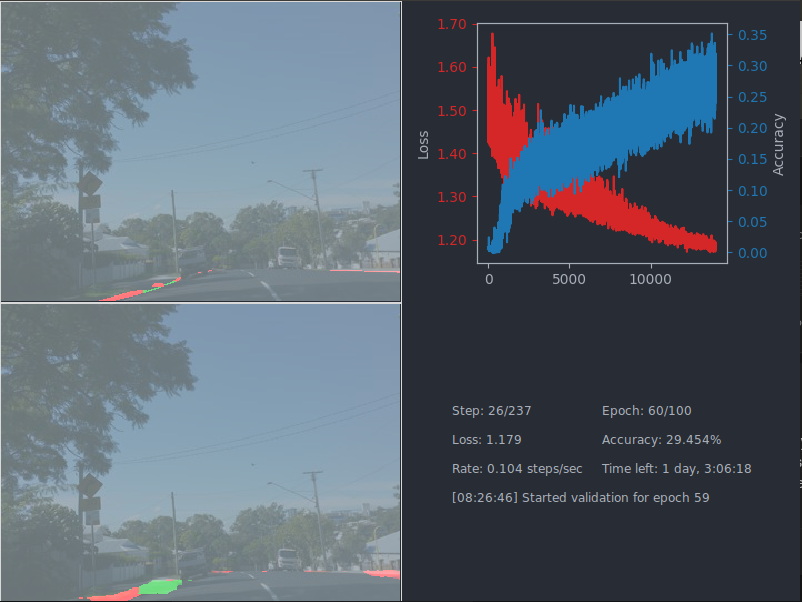
\includegraphics[width=\linewidth]{figures/experiments/gui.png}
		\caption[Training GUI]{A screen capture of the GUI that was used to visualize training results. In clockwise from the top left, the GUI visualizes the ground truth data, a live plot of the loss and accuracy, various statistics, and the network output.}
		\label{fig:experiments-gui}
	\end{subfigure}
	\hfill
	\begin{subfigure}{0.45\textwidth}
		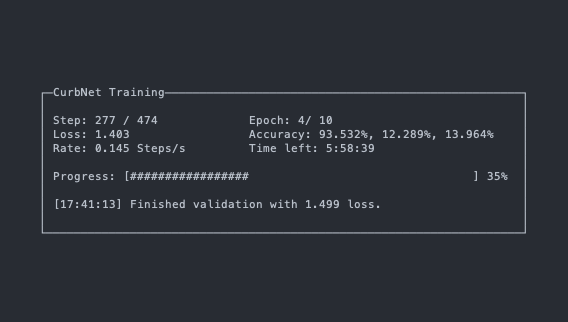
\includegraphics[width=\linewidth]{figures/experiments/cli.png}
		\caption[Training CLI]{A screen capture of the CLI that was used to train the network remotely.}
		\label{fig:experiments-cli}
	\end{subfigure}
	\caption[Training UI]{The two available user interfaces available to use with CurbNet. The GUI was mean to more simply and quickly deliver the most important information first to the researcher. The CLI was designed to allow training status along with the most pertinent information to be shown remotely with little overhead.}
\end{figure}

The different components necessary to train the network are written in such a way as to be modular, with nearly everything being easily configurable.
For example, the network, optimizer, and loss criterion can easily be swapped by changing command-line arguments or parameters in the JSON file.
This makes running different experiments straightforward.

\section{Results}\label{section:experiments-results}
Running our network with the tuned hyperparameters chosen by the hyperparameter search in Section \ref{section:experiments-hyperparameters} for 30,336 iterations, we were able to achieve a mIoU accuracy of 50.188\% on the validation dataset.

\begin{table}[]
	\centering
\begin{tabular}{@{}crrrrrr@{}}
	\toprule
	& \multicolumn{5}{c}{IoU} &  \\ \cmidrule(lr){2-6}
	Dataset & Curb & Curb Cut & Road & Sidewalk & Ignore & mIoU \\ \midrule
	Training & 24.219\% & 28.064\% & 83.372\% & 31.523\% & 95.673\% & 52.570\% \\
	Validation & 22.987\% & 25.292\% & 79.942\% & 28.587\% & 94.131\% & 50.188\% \\ \bottomrule
\end{tabular}
\caption[Network Results]{Results after training the network for 30,366 iterations on the Mapillary Vistas dataset \cite{mapillary} and evaluating it against both the training and validation datasets using IoU. The network achieves higher accuracy on the training dataset than on the validation dataset, but did not overfit on the training set.}
\label{tab:mapillary-results}
\end{table}

The network is able to produce the segmentations seen in \figref{fig:experiments-resultsmapillary}.
We also notice that the network is able to achieve very high IoU accuracy for the road class, as seen in \tabref{tab:mapillary-results}.
This is due to the original purpose of DeepLab v3+ as a road segmentation network \cite{deeplab}.
The IoU accuracy of curbs, curb cuts, and sidewalks are lower than of the road class.
One possible reason for this is that IoU is especially hard to fulfill when there are only a few pixels belonging to the class.
Cases where the class has only a few pixels and the borders do not match exactly would return a low IoU.

\begin{figure}
	\centering
	\begin{subfigure}{.45\textwidth}
		\centering
		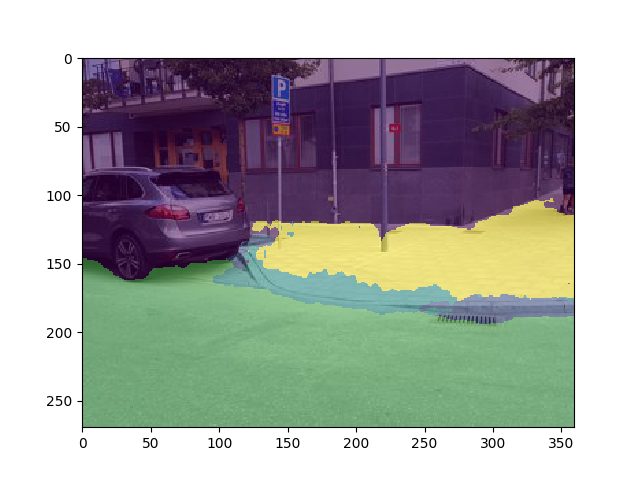
\includegraphics[width=\linewidth]{figures/experiments/results-mapillary/1.png}
		\caption[Mapillary Vistas Segmentation Result 1]{}
		\label{fig:mapresult-1}
	\end{subfigure}
	\hfill
	\begin{subfigure}{.45\textwidth}
		\centering
		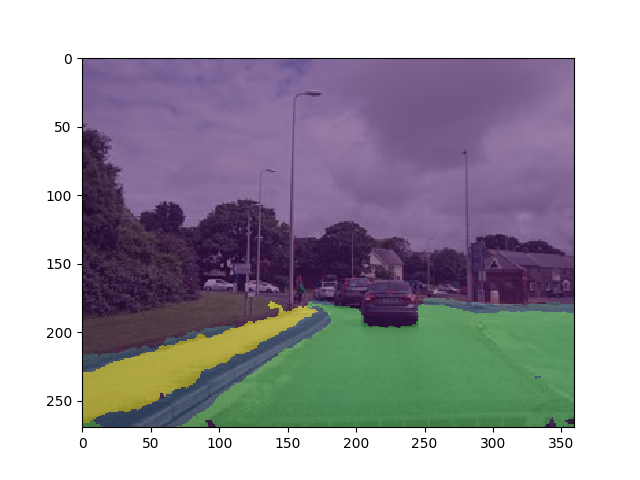
\includegraphics[width=\linewidth]{figures/experiments/results-mapillary/2.png}
		\caption[Mapillary Vistas Segmentation Result 2]{}
		\label{fig:mapresult-2}
	\end{subfigure}
	
	\vspace{12pt}%------------
	
	\begin{subfigure}{.45\textwidth}
		\centering
		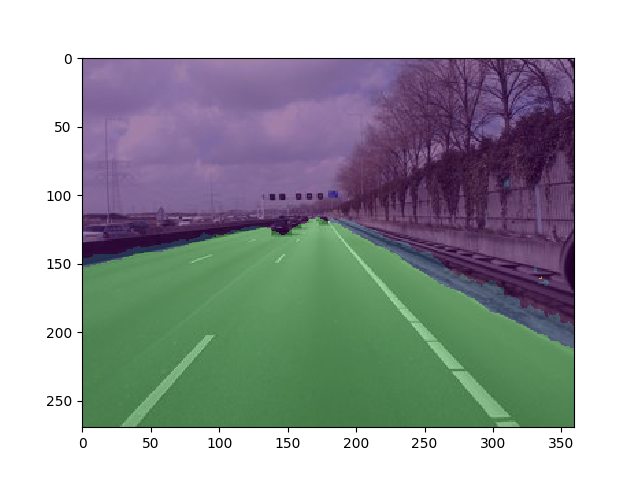
\includegraphics[width=\linewidth]{figures/experiments/results-mapillary/3.png}
		\caption[Mapillary Vistas Segmentation Result 3]{}
		\label{fig:mapresult-3}
	\end{subfigure}
	\hfill
	\begin{subfigure}{.45\textwidth}
		\centering
		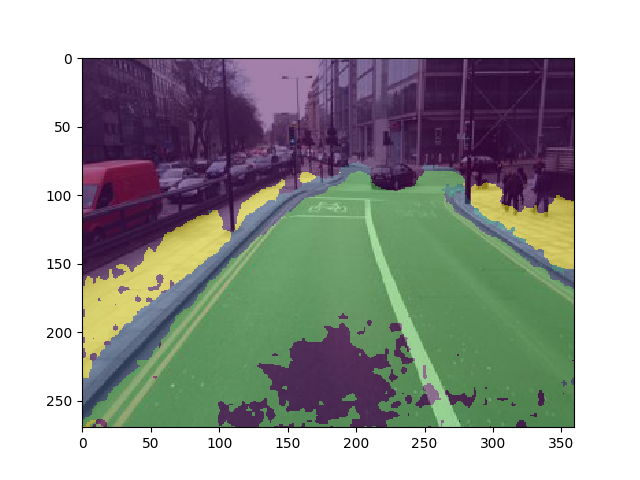
\includegraphics[width=\linewidth]{figures/experiments/results-mapillary/4.png}
		\caption[Mapillary Vistas Segmentation Result 4]{}
		\label{fig:mapresult-4}
	\end{subfigure}

	\vspace{12pt}%------------
	
	\begin{subfigure}{.45\textwidth}
		\centering
		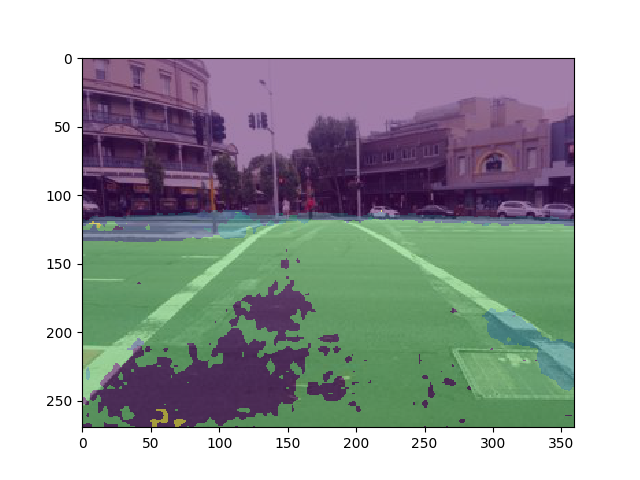
\includegraphics[width=\linewidth]{figures/experiments/results-mapillary/5.png}
		\caption[Mapillary Vistas Segmentation Result 5]{}
		\label{fig:mapresult-5}
	\end{subfigure}
	\hfill
	\begin{subfigure}{.45\textwidth}
		\centering
		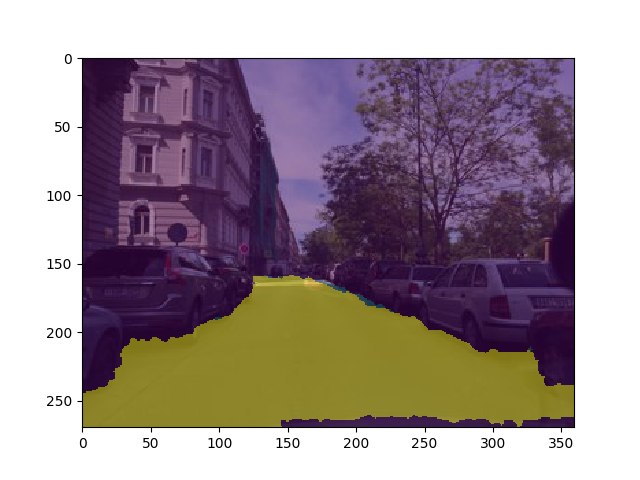
\includegraphics[width=\linewidth]{figures/experiments/results-mapillary/6.png}
		\caption[Mapillary Vistas Segmentation Result 6]{}
		\label{fig:mapresult-6}
	\end{subfigure}

	\caption[Mapillary Vistas Segmentation Results]{A sample of some segmentation results from the trained CurbNet model. The images are from the Mapillary Vistas dataset \cite{mapillary}. Green is road, yellow is sidewalk, blue is curb, turquoise is curb cuts, and purple is the ignore class. Figure \ref{fig:mapresult-1} shows how the model is able to identify all of the different traversibility classes. Figures \ref{fig:mapresult-2} and \ref{fig:mapresult-3} shows that segmentation of curbs even in the distance can be performed well. Figures \ref{fig:mapresult-4} and \ref{fig:mapresult-5} shows that curb cuts in the distance are also identified and segmented by the network, although sometimes roads are mislabeled as ignore. Figure \ref{fig:mapresult-5} also shows a failure case where some road markings in the bottom right corner have been mislabeled as curb. Figure \ref{fig:mapresult-6} shows a case where the entire road is labeled as sidewalk.}
	\label{fig:experiments-resultsmapillary}
\end{figure}
\begin{figure}
	\centering
	\begin{subfigure}{.45\textwidth}
		\centering
		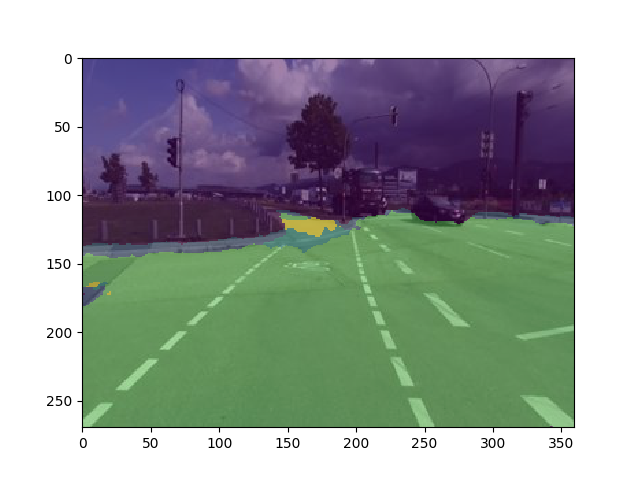
\includegraphics[width=\linewidth]{figures/experiments/results-obelix/1.png}
		\caption[Obelix Segmentation Result 1]{}
		\label{fig:obresult-1}
	\end{subfigure}
	\hfill
	\begin{subfigure}{.45\textwidth}
		\centering
		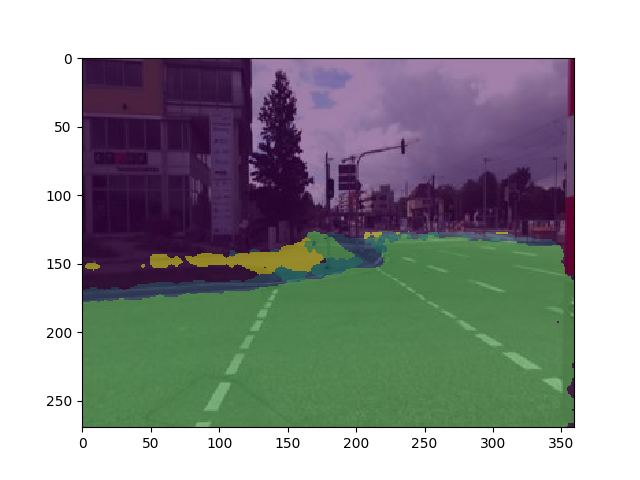
\includegraphics[width=\linewidth]{figures/experiments/results-obelix/2.png}
		\caption[Obelix Segmentation Result 2]{}
		\label{fig:obresult-2}
	\end{subfigure}
	
	\vspace{12pt}%------------
	
	\begin{subfigure}{.45\textwidth}
		\centering
		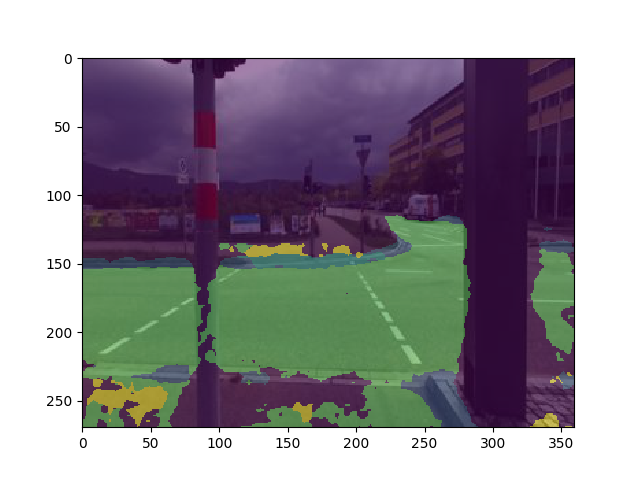
\includegraphics[width=\linewidth]{figures/experiments/results-obelix/3.png}
		\caption[Obelix Segmentation Result 3]{}
		\label{fig:obresult-3}
	\end{subfigure}
	\hfill
	\begin{subfigure}{.45\textwidth}
		\centering
		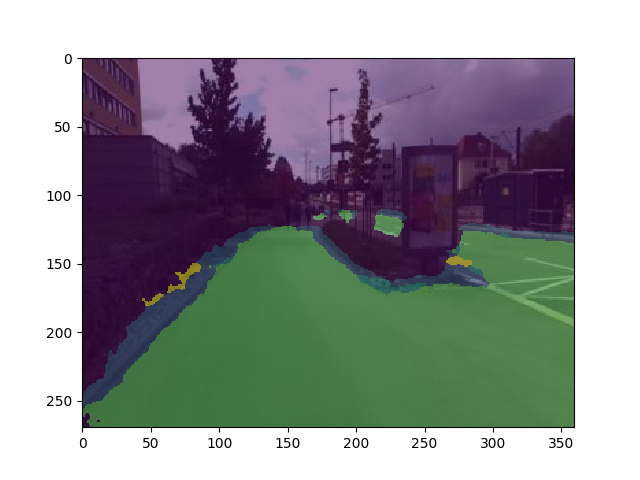
\includegraphics[width=\linewidth]{figures/experiments/results-obelix/4.png}
		\caption[Obelix Segmentation Result 4]{}
		\label{fig:obresult-4}
	\end{subfigure}

	\vspace{12pt}%------------
	
	\begin{subfigure}{.45\textwidth}
		\centering
		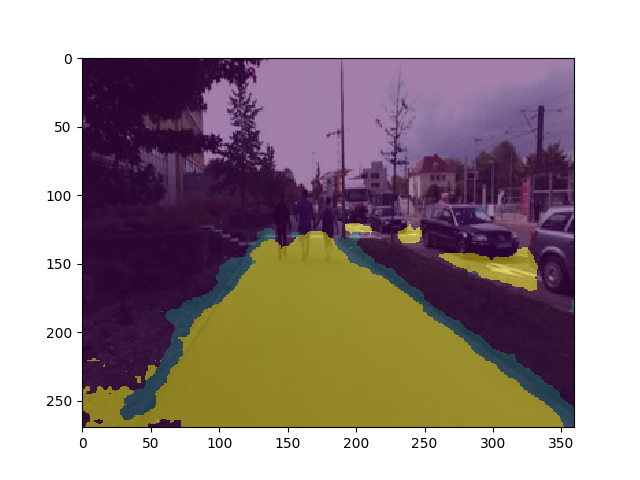
\includegraphics[width=\linewidth]{figures/experiments/results-obelix/5.png}
		\caption[Obelix Segmentation Result 5]{}
		\label{fig:obresult-5}
	\end{subfigure}
	\hfill
	\begin{subfigure}{.45\textwidth}
		\centering
		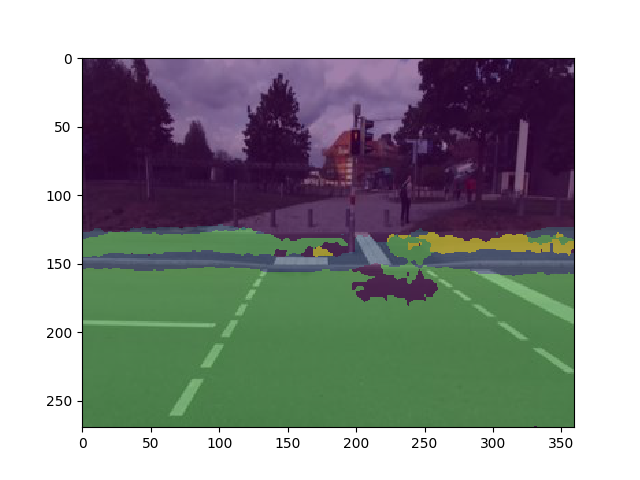
\includegraphics[width=\linewidth]{figures/experiments/results-obelix/6.png}
		\caption[Obelix Segmentation Result 6]{}
		\label{fig:obresult-6}
	\end{subfigure}

	\caption[Obelix Segmentation Results]{A sample of some segmentation results from the trained CurbNet model. The images are from the Obelix dataset. Green is road, yellow is sidewalk, blue is curb, turquoise is curb cuts, and purple is the ignore class. Figures \ref{fig:obresult-1} and \ref{fig:obresult-2} shows how the model is able to identify all of the different traversibility classes in the Obelix dataset even though it was only trained on the Mapillary dataset. Figure \ref{fig:obresult-3} shows curb cuts are sometimes also identified properly, as seen in the identification of the curb cut across the street, but not always, as seen in the curb cut directly in front of Obelix. Figures \ref{fig:obresult-4} and \ref{fig:obresult-5} shows a case where the network seems to be unable to decide if the sidewalk is a sidewalk or a road. In both cases, the sidewalk edge is marked as a curb, when it should not. Figure \ref{fig:obresult-6} shows a case where the left half of the sidewalk is labeled as road while the right half is labeled as sidewalk.}
	\label{fig:experiments-resultsobelix}
\end{figure}

In these results we can observe that the network is quite capable of identifying each of the traversability classes.
\figref{fig:mapresult-1} shows an example of how the network is able to identify each of the traversibility classes.
The network can also identify traversability classes, specifically curbs and curb cuts, which are in the distance and thus have a relatively small size, as can be observed in Figures \ref{fig:mapresult-2} - \ref{fig:mapresult-5}.
In these cases, the segmentation is significantly larger than the size of the curb itself, i.e. even though the intersection is significant, there is a significant area around the curb that is falsely identified as also being a part of the curb.
Figure \ref{fig:mapresult-5} shows a failure case where the road marking in the bottom right corner is mislabeled as a curb.
Figures \ref{fig:mapresult-4} and \ref{fig:mapresult-5} also show failure cases where the road is labeled as the ignore class.
Figure \ref{fig:mapresult-6} shows another failure case where the entire road is mislabeled as sidewalk.

We also ran inference against a dataset gathered by the onboard cameras on the Obelix robot using the network.
The results of this experiment can be seen in \figref{fig:experiments-resultsobelix}.
Figures \ref{fig:obresult-1} and \ref{fig:obresult-2} show that the network is able to generalize to the Obelix dataset and is able to identify the different traversability classes in the images, despite never having been trained on them.
Figure \ref{fig:obresult-3} shows although curb cuts are correctly identified, as in the case of the curb cut across the street, they are also sometimes mislabeled, as in the case of the curb cut directly ahead of the robot.
We can observe in Figures \ref{fig:obresult-4} and \ref{fig:obresult-5} that the network seems unable to decide whether the asphalt sidewalk is a road or a sidewalk.
The same failure case can be seen in Figure \ref{fig:obresult-6} where the left side of the sidewalk is mislabeled as road while the right side is labeled correctly as sidewalk.

We observe that the main failure cases of the network are falsely identifying certain road markings as curbs and identifying certain roads as sidewalks or vice versa.
Certain road markings which are located near road edges are sometimes segmented as curbs, as can be seen in the bottom right corner of \figref{fig:mapresult-5}.
We believe that this is due to the texture of the marking being colored similarly to some curbs as well as its shape which does resemble a curb.
In some cases, the sidewalk is identified as a road, as in \figref{fig:obresult-5} or the entire road is identified as a sidewalk, as in \figref{fig:mapresult-6}.
We believe that this may occur when sidewalks have an asphalt-like texture, as in the case in \figref{fig:obresult-5}.
